\documentclass[12pt,a4paper]{article}

%\usepackage[left=1.5cm,right=1.5cm,top=1cm,bottom=2cm]{geometry}
\usepackage[in, plain]{fullpage}
\usepackage{array}
%\usepackage{../../pas-math}
\usepackage{../../moncours}



%-------------------------------------------------------------------------------
%          -Packages nécessaires pour écrire en Français et en UTF8-
%-------------------------------------------------------------------------------
\usepackage[utf8]{inputenc}
\usepackage[frenchb]{babel}
%\usepackage{numprint}
\usepackage[T1]{fontenc}
%\usepackage{lmodern}
\usepackage{textcomp}
\usepackage[french, boxed]{algorithm2e}
\usepackage{hyperref}


%-------------------------------------------------------------------------------

%-------------------------------------------------------------------------------
%                          -Outils de mise en forme-
%-------------------------------------------------------------------------------
\usepackage{hyperref}
\hypersetup{pdfstartview=XYZ}
%\usepackage{enumerate}
\usepackage{graphicx}
\usepackage{multicol}
\usepackage{tabularx}
\usepackage{multirow}
\usepackage{color}
\usepackage{eurosym}


\usepackage{anysize} %%pour pouvoir mettre les marges qu'on veut
%\marginsize{2.5cm}{2.5cm}{2.5cm}{2.5cm}

\usepackage{indentfirst} %%pour que les premier paragraphes soient aussi indentés
\usepackage{verbatim}
\usepackage{enumitem}
\usepackage{booktabs}
\usepackage[usenames,dvipsnames,svgnames,table]{xcolor}

\usepackage{variations}

%-------------------------------------------------------------------------------


%-------------------------------------------------------------------------------
%                  -Nécessaires pour écrire des mathématiques-
%-------------------------------------------------------------------------------
\usepackage{amsfonts}
\usepackage{amssymb}
\usepackage{amsmath}
\usepackage{amsthm}
\usepackage{tikz}
\usepackage{xlop}
\usepackage[output-decimal-marker={,}]{siunitx}
%-------------------------------------------------------------------------------

%-------------------------------------------------------------------------------
%                  -Nécessaires pour écrire des formules chimiquess-
%-------------------------------------------------------------------------------

\usepackage[version=4]{mhchem}

%-------------------------------------------------------------------------------
% Pour pouvoir exploiter les fichiers directement dans beamer
\newcommand{\pause}{\ }
%-------------------------------------------------------------------------------
%                    - Mise en forme avancée
%-------------------------------------------------------------------------------

\usepackage{ifthen}
\usepackage{ifmtarg}


\newcommand{\ifTrue}[2]{\ifthenelse{\equal{#1}{true}}{#2}{$\qquad \qquad$}}

%\newcommand{\kword}[1]{\textcolor{red}{\underline{#1}}}
%-------------------------------------------------------------------------------

%-------------------------------------------------------------------------------
%                     -Mise en forme d'exercices-
%-------------------------------------------------------------------------------
%\newtheoremstyle{exostyle}
%{\topsep}% espace avant
%{\topsep}% espace apres
%{}% Police utilisee par le style de thm
%{}% Indentation (vide = aucune, \parindent = indentation paragraphe)
%{\bfseries}% Police du titre de thm
%{.}% Signe de ponctuation apres le titre du thm
%{ }% Espace apres le titre du thm (\newline = linebreak)
%{\thmname{#1}\thmnumber{ #2}\thmnote{. \normalfont{\textit{#3}}}}% composants du titre du thm : \thmname = nom du thm, \thmnumber = numéro du thm, \thmnote = sous-titre du thm

%\theoremstyle{exostyle}
%\newtheorem{exercice}{Exercice}
%
%\newenvironment{questions}{
%\begin{enumerate}[\hspace{12pt}\bfseries\itshape a.]}{\end{enumerate}
%} %mettre un 1 à la place du a si on veut des numéros au lieu de lettres pour les questions 
%-------------------------------------------------------------------------------

%-------------------------------------------------------------------------------
%                    - Mise en forme de tableaux -
%-------------------------------------------------------------------------------

\renewcommand{\arraystretch}{1.7}

\setlength{\tabcolsep}{1.2cm}

%-------------------------------------------------------------------------------



%-------------------------------------------------------------------------------
%                    - Racourcis d'écriture -
%-------------------------------------------------------------------------------
%Droites
\newcommand{\dte}[1]{$(#1)$}
\newcommand{\fig}[1]{figure $#1$}
\newcommand{\sym}{symétrique}
\newcommand{\syms}{symétriques}
\newcommand{\asym}{axe de symétrie}
\newcommand{\asyms}{axes de symétrie}
\newcommand{\seg}[1]{$[#1]$}
\newcommand{\monAngle}[1]{$\widehat{#1}$}
\newcommand{\bissec}{bissectrice}
\newcommand{\mediat}{médiatrice}
\newcommand{\ddte}[1]{$[#1)$}


% Angles orientés (couples de vecteurs)
\newcommand{\aopp}[2]{(\vec{#1}, \vec{#2})} %Les deuc vecteurs sont positifs
\newcommand{\aopn}[2]{(\vec{#1}, -\vec{#2})} %Le second vecteur est négatif
\newcommand{\aonp}[2]{(-\vec{#1}, \vec{#2})} %Le premier vecteur est négatif
\newcommand{\aonn}[2]{(-\vec{#1}, -\vec{#2})} %Les deux vecteurs sont négatifs

%Ensembles mathématiques
\newcommand{\naturels}{\mathbb{N}} %Nombres naturels
\newcommand{\relatifs}{\mathbb{Z}} %Nombres relatifs
\newcommand{\rationnels}{\mathbb{Q}} %Nombres rationnels
\newcommand{\reels}{\mathbb{R}} %Nombres réels
\newcommand{\complexes}{\mathbb{C}} %Nombres complexes


%Intégration des parenthèses aux cosinus
\newcommand{\cosP}[1]{\cos\left(#1\right)}
\newcommand{\sinP}[1]{\sin\left(#1\right)}


%Probas stats
\newcommand{\stat}{statistique}
\newcommand{\stats}{statistiques}


\newcommand{\homo}{homothétie}
\newcommand{\homos}{homothéties}


\newcommand{\mycoord}[3]{(\textcolor{red}{\num{#1}} ; \textcolor{Green}{\num{#2}} ; \textcolor{blue}{\num{#3}})}
%-------------------------------------------------------------------------------

%-------------------------------------------------------------------------------
%                    - Mise en page -
%-------------------------------------------------------------------------------

\newcommand{\twoCol}[1]{\begin{multicols}{2}#1\end{multicols}}


\setenumerate[1]{font=\bfseries,label=\textit{\alph*})}
\setenumerate[2]{font=\bfseries,label=\arabic*)}


%-------------------------------------------------------------------------------
%                    - Elements cours -
%-------------------------------------------------------------------------------

%Correction d'exercice
\newcommand{\exoSec}[2]{\subsection*{Exercice #1 page #2}}
%-------------------------------------------------------------------------------
%                    - raccourcis d'écriture -
%-------------------------------------------------------------------------------

%Mise en évidence de termes clés
\newcommand{\mykw}[1]{\textcolor{red}{\underline{\textbf{#1}}}}

%Exercices
\newcommand{\exo}[2]{exercice #1 page #2}
\newcommand{\Exo}[2]{Exercice #1 page #2}

\renewcommand{\pause}{\ }

%Intervalles
\newcommand{\interOO}[2]{$]$#1 , #2$[$}
\newcommand{\interOF}[2]{$]$#1 , #2$]$}
\newcommand{\interFO}[2]{$[$#1 , #2$[$}
\newcommand{\interFF}[2]{$[$#1 , #2$]$}





\date{}
\title{}


\begin{document}
	
	
\chap[num=4, color=blue]{Circuit électrique}{Olivier FINOT, \today }	

\section{\'Eléments d'un circuit électrique}

%\begin{myact}{1 page 110-111}
%	\begin{enumerate}
%		\item Les grands réservoirs d'eau visibles sur ces documents sont \kw{les océans} et \kw{la banquise}.
%		\item Les palmiers arrivent à pousser en plein désert car \kw{ils ont de faibles besoins en eau}.
%		\item Les boissons nous sont nécessaires pour \kw{renouveler l'eau dans notre corps}.
%		\item \kw{Le c\oe ur} est l'organe du corps humain qui contient le plus d'eau.
%		\item \kw{La peau} est l'organe du corps humain qui contient le moins d'eau.
%	\end{enumerate}
%\end{myact}




\begin{center}
	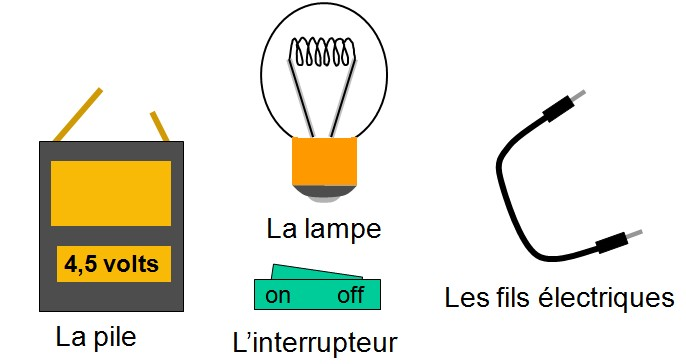
\includegraphics[scale=0.8]{img/dipoles}
\end{center}



\begin{mybilan}
	\begin{itemize}
		\item La pile est une \kw{source d'énergie}, c'est elle qui produit le courant électrique dans le circuit.
		\item La lampe est un \kw{récepteur}, elle utilise le courant produit par le générateur pour produire de l'énergie lumineuse.
		\item L'interrupteur est un \kw{élément de commande} du circuit, il permet de le fermer ou de l'ouvrir.
		\item Les fils électriques permettent la \kw{liaison} entre les différents éléments du circuit.
		
	\end{itemize}

On appelle \kw{dipôle électrique}, un composant électrique comportant deux bornes. La pile et la lampe sont des dipôles

\end{mybilan}

\newpage 

\section{Réalisation d'un circuit simple}

Expérience : on dispose d'une pile, d'un interrupteur, d'une lampe et de fils de connexion.

Réalisons le circuit dans lequel la lampe est commandée par un interrupteur.

\begin{center}
	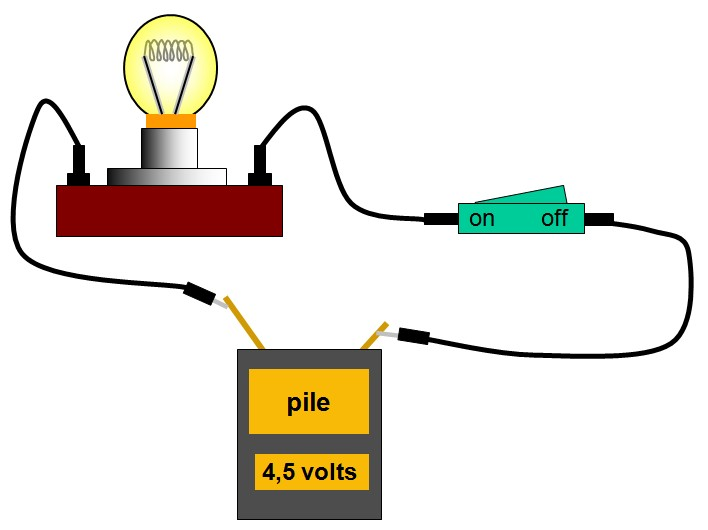
\includegraphics[scale=0.5]{img/circuitsimple}
\end{center}

\begin{mybilan}
	\begin{itemize}
		\item Un circuit électrique simple est formé par une \kw{boucle} qui comporte une \kw{source d'énergie}, un \kw{interrupteur}, un \kw{dipôle récepteur} (ex : une lampe) reliés par des \kw{fils de connexion.}
		
		\item Si la lampe brille, \kw{le courant électrique circule} : on dit que le circuit est \kw{fermé}.
		
		\item Si la lampe est éteinte, \kw{le courant ne circule plus} : on dit que le circuit est \kw{ouvert}.
		
		
	\end{itemize}
\end{mybilan}

\section{Schéma normalisé}

\begin{mybilan}
	Pour <<dessiner>> un circuit, il a été convenu d'une même représentation utilisée par tous.

	\begin{itemize}
		\item Chaque élément d'un circuit est représenté par son \kw{symbole normalisé}.
		\item On dit que l'on représente le circuit par un \kw{schéma électrique}.
	\end{itemize}

\end{mybilan}

\begin{mymeth}
	\begin{enumerate}
		\item On dessine un rectangle au crayon;
		\item On efface les endroits où seront placés les éléments (aucun élément n'est placé dans un coin du circuit);
		\item On place les symboles des différents éléments
	\end{enumerate}
\end{mymeth}


\begin{myex}
	Schéma du circuit vu au II. :
	\begin{center}
		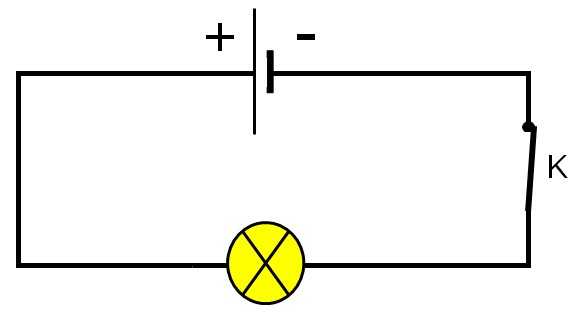
\includegraphics[scale=0.6]{img/schema}
	\end{center}
\end{myex}

\section{Court-crcuit}

\underline{Expérience} : On réalise le montage suivant :

\begin{center}
	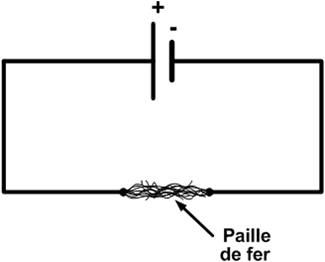
\includegraphics[scale=0.5]{img/courtcircuit}
\end{center}

\underline{Observation} : Lorsqu'on ferme le circuit, la paille de fer brule.

\underline{Interprétation} :

\begin{itemize}
	\item Les bornes de la pile sont directement reliées entre elles sans aucun dipôles : on dit que la pile est en \kw{court-circuit}.
	\item Dans ce cas, le courant devient très intense et échauffe fortement la paille de fer jusqu'à ce qu'elle brûle.
\end{itemize}

\underline{Conclusion}

\begin{mybilan}
	\begin{itemize}
		\item Dans un montage, il y a \kw{court-circuit} quand les \kw{deux bornes de la source d'énergie sont directement reliées} par des fils de connexion.
		\item Un court-circuit présente un \kw{danger d'incendie et de destruction de la source d'énergie}
	\end{itemize}
\end{mybilan}
%\appendix

%\newpage


\end{document}]